\documentclass{article}

% if you need to pass options to natbib, use, e.g.:
%     \PassOptionsToPackage{numbers, compress}{natbib}
% before loading neurips_2019

% ready for submission
% \usepackage{neurips_2019}

% to compile a preprint version, e.g., for submission to arXiv, add add the
% [preprint] option:
%     \usepackage[preprint]{neurips_2019}

% to compile a camera-ready version, add the [final] option, e.g.:
     \usepackage[final]{neurips_2019}

% to avoid loading the natbib package, add option nonatbib:
%     \usepackage[nonatbib]{neurips_2019}

\usepackage[utf8]{inputenc} % allow utf-8 input
\usepackage[T1]{fontenc}    % use 8-bit T1 fonts
\usepackage{hyperref}       % hyperlinks
\usepackage{url}            % simple URL typesetting
\usepackage{booktabs}       % professional-quality tables
\usepackage{amsfonts}       % blackboard math symbols
\usepackage{nicefrac}       % compact symbols for 1/2, etc.
\usepackage{microtype}      % microtypography

\usepackage{graphicx}
\usepackage{subfig}

\title{AI Learning Report}

% The \author macro works with any number of authors. There are two commands
% used to separate the names and addresses of multiple authors: \And and \AND.
%
% Using \And between authors leaves it to LaTeX to determine where to break the
% lines. Using \AND forces a line break at that point. So, if LaTeX puts 3 of 4
% authors names on the first line, and the last on the second line, try using
% \AND instead of \And before the third author name.

\author{%
  YiFei LIU, Zhining JIANG, Jing WAN, Lingxi ZHANG, Yuxin ZHANG \\
  Department of Science\\
  Financial Mathematics\\
  Hong Kong University of Science and Technology\\
  % examples of more authors
  % \And
  % Coauthor \\
  % Affiliation \\
  % Address \\
  % \texttt{email} \\
  % \AND
  % Coauthor \\
  % Affiliation \\
  % Address \\
  % \texttt{email} \\
  % \And
  % Coauthor \\
  % Affiliation \\
  % Address \\
  % \texttt{email} \\
  % \And
  % Coauthor \\
  % Affiliation \\
  % Address \\
  % \texttt{email} \\
}

\begin{document}

\maketitle

\begin{abstract}
 The whole report contains 4 parts. The first part is the reflection on an AI article "Natural Language Processing in Accounting Auditing and Finance: A Synthesis of the Literature with a Roadmap for Future Research" which synthesizes the extant literature in NLP in accounting, auditing and finance to establish the state of current knowledge. The second part is AI technology applied in company research, we choose SenseTime technology as our research object and tried to analysis it from its management team, financial profit predict, scientific research ability and products response in the market. The third part is the suggestion for further study. The fourth part is individual contribution.
\end{abstract}

\section{Progress and Learning}
\subsection{Learning and Progress from the Topic Company Seniors}
\subsubsection{The first stage - basic information gathering}
The main goal of the first phase is:
\begin{itemize}
	\item Understand the basic information of the entire corporate executives, including academic background, academic achievements, and development process.
	\item The overall situation of obtaining the employees of SenseTime in LinkedIn China mainly includes the distribution of employees, the distribution of employees' colleges and universities, and the distribution of employees.
\end{itemize}

The main result of the first phase is:
\begin{itemize}
	\item[1.] The management team is generally from the top universities in the world, and has rich academic achievements and strong scientific research in the field of image recognition.
	\item[2.] SenseTime Technology employees generally graduated from key universities around the world. The sample of employees from domestic 985 universities accounted for more than 41\%, and the number of doctors exceeded 60. The personnel are mainly distributed in Beijing and Shenzhen. Researchers account for a large proportion, with researchers and engineers in the sample accounting for more than 31\%.
\end{itemize}
\begin{figure}[htb]
	\centering
	\subfloat[Employee area distribution.]{
		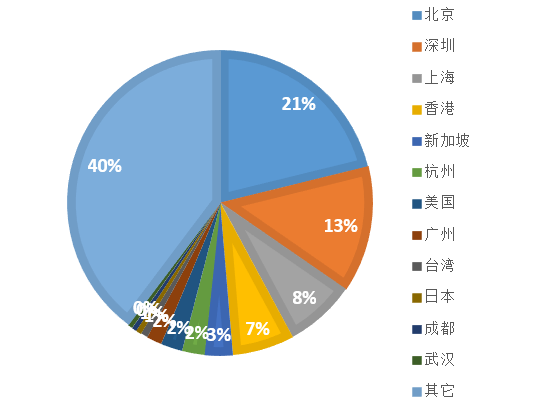
\includegraphics[width=1.6in]{yuangong_diqu.png}}
	%\hspace{0.1in}
	\subfloat[Employee graduation college distribution.]{
		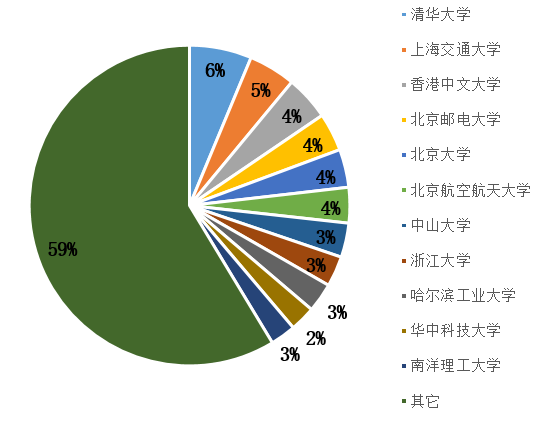
\includegraphics[width=1.6in]{yuangong_yuanxiao.png}}
	%\hspace{0.1in}
	\subfloat[Employee position distribution.]{
		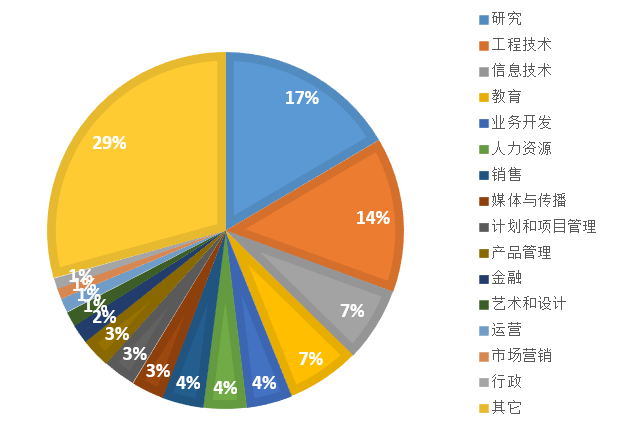
\includegraphics[width=1.8in]{yuangong_zhiwei.png}}
	\caption{Basic information gathering.}
\end{figure}

\subsubsection{The second stage - crawler}
Since the company information is constantly updated and there are many management personnel, it is obviously time-consuming and labor-intensive to collect information one by one at regular intervals.
And the latest information update of the company is not timely, which may lead to wrong judgment of the company, so the goal of the second stage is: learning crawler technology.
We attempt to capture relevant news of the company from the macro level, the industry level, the capital market, and the company level.

The implementation process is:
\begin{itemize}
	\item[1.] Determine the site segments to be crawled and classify them into four aspects: macro, industry, company, and capital market.The finalized websites include Securities Times, Hexun.com, Eastern Fortune.com, the financial sector, and Zhongcai.com, and finally decided to climb nearly 20 websites.
	\item[2.] Based on BeautifulSoup framework, craw news from these static websites, Get the title, publish time.
	\item[3.] Use multi-threading to allow crawlers of different web pages to execute concurrently to shorten crawling time.
\end{itemize}
\begin{figure}[htb]
	\centering
	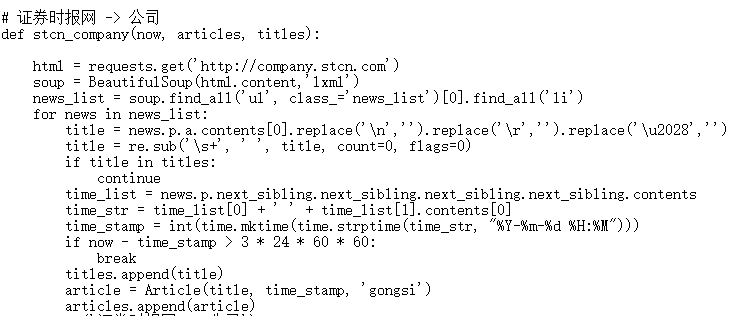
\includegraphics[width=5in]{code_example.png}
	\caption{Code (example).}
\end{figure}

\subsubsection{The third stage - word segmentation and clustering}
Due to the large number of titles taken out, the key information needs to be extracted and stored in an Excel table, updated once a day.
The goal of this stage is to extract information from the crawled content, store the content in the excel table, update it daily, and form the word cloud of the recently updated day into a word cloud for visual display.
The implementation process is:
\begin{itemize}
	\item[1.] Identify the keywords you want to crawl.
	\item[2.] Crawl once a day, word segmentation of the title taken every day
	\item[3.] Using TF/IDF algorithm to count the five words with the highest frequency of words after adjustment, as key information. TF-IDF algorithm: The words that appear most frequently in the article are not necessarily keywords, such as the common stop words that do not make much sense to the article itself. IDF (Inverse Document Frequency) is inversely proportional to the commonality of a word. Multiply the word frequency (TF) and IDF to get the TF-IDF value of a word. The higher the importance of a word to an article, the greater its TF-IDF value, so the first several words are the keywords of the article.
	\item[4.] Compare the key information extracted in the latest day with the key information of the previous day. If the extracted key information overlaps more than 60\%, it means that there is no information update on the current day. If it does not exceed 60\%, the new information appears to be updated, and the extracted key information and time are updated in the excel form.
	\item[5.] Visualize and display the word cloud for news of all keywords updated on the latest day.
\end{itemize}

\begin{figure}[htb]
	\centering
	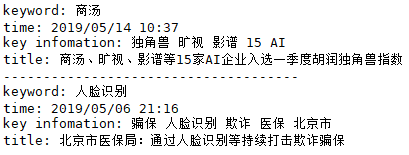
\includegraphics[width=4in]{output_screen.png}
	\caption{Output in screen}
\end{figure}

\begin{figure}[htb]
	\centering
	
\includegraphics[width=3.5in]{word_cloud.png}
	\caption{Wordcloud}
\end{figure}

\begin{figure}[htb]
	\centering
	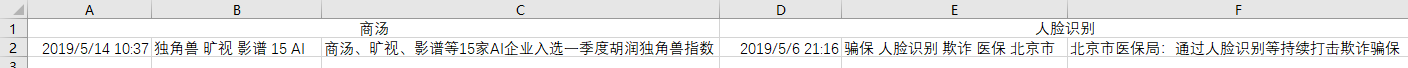
\includegraphics[width=5in]{output_excel.png}
	\caption{Output in excel}
\end{figure}
\subsection{Learning and Progress from the Topic Revenue Forecast Based on Machine Learning Algorithm}
Throughout this semester, our team conducted in-depth research on SenseTime Technology. In the process, I quickly improved my ability in artificial intelligence (programming ability). After learning the crawlers with my teammates, since SenseTime Technology itself has almost no data, after obtaining the teacher's consent, I searched for Zhongqingbao, a listed technology company in the same field as SenseTime Technology, and downloaded its stock’s closing price for recent five years through WIND. I intend to use machine learning to predict the price of the stock in the future. First of all, because MATLAB has the packaged ML, which is very convenient to use, I chose MATLAB as my programming language. Use Sample Partial Auto-correlation function and find the Sample Partial Auto-correlation are almost above 0.3 and some reach 0.5.To make the model more concise,I choose Auto-regressive model. 

Then I come to the most important part: Creating the network. The core idea of building a network is to change the number of layers and structural parameters so as to make the final error curve minimized. The network structure as shown in figure 6.Then adjust the training data and test data ratio, MATLAB defaults to 70:15:15.Finally, the ideal error curve(figure 7) and forecast curve of stock's price(figure 7) are obtained.
\begin{figure}[htb]
    \centering
    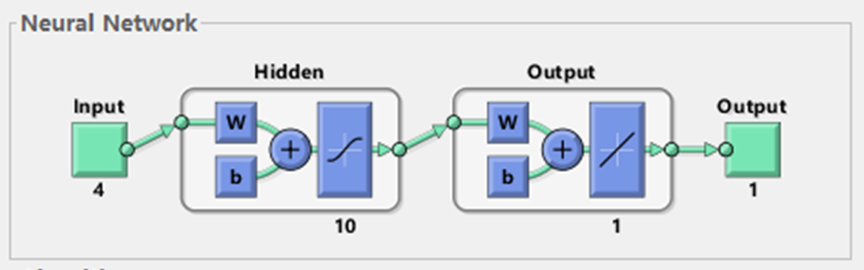
\includegraphics[width=4in]{ml1.png}
  	\caption{Network Structure}
\end{figure}
\begin{figure}[htb]
	\centering
	\subfloat[Best Validation Performance]{
		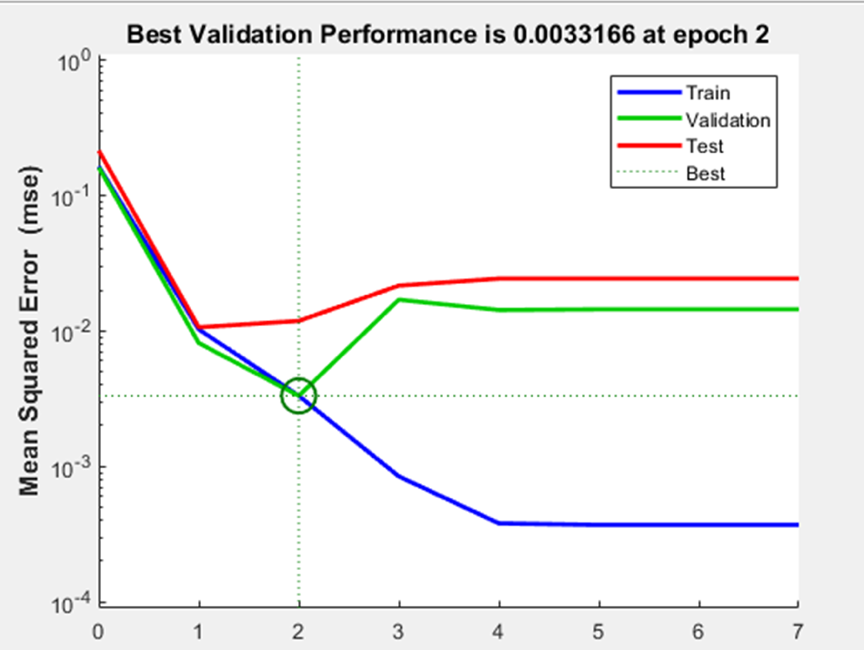
\includegraphics[width=1.6in]{ml2.png}}
	%\hspace{0.1in}
	\subfloat[The Forecast Curve of Stock’s Price]{
		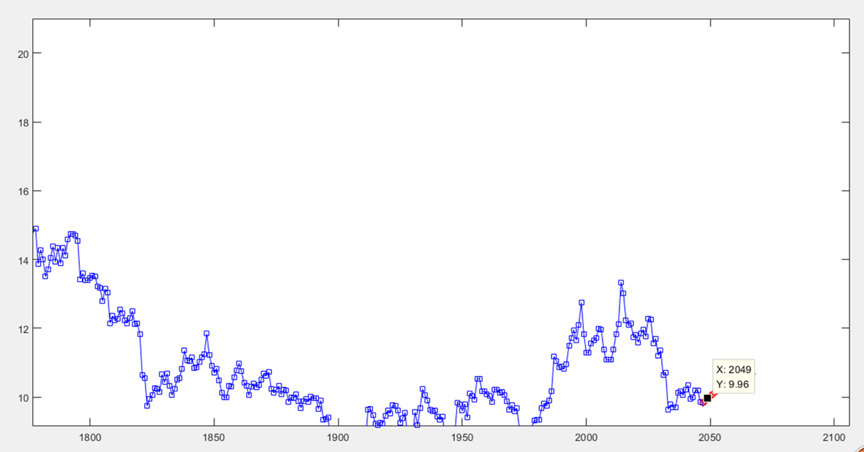
\includegraphics[width=1.6in]{ml3.png}}
	\caption{Basic information gathering}
\end{figure}
\subsection{Learning and Progress from the Topic Analyzing Sense Time’s Academic Performance}
Since SenseTime is a technology-driven company, fruitful academic achievements are one of its key competitiveness. I want to get a better understanding of Sense Time’s development prospect through the published papers and books.  At the beginning, I used Excel’s formulas to process the text including citation, publication information that copied and pasted from google scholar into different columns to make them become formatted. Then I used formulas like SUMIF, VlOOLUP to find and sort the papers published on top journals to get a deeper understanding of Sense Time’s academic performance. But then I tried to use python to help me crawl the information from google scholar more efficiently and automatically. There many different packets, like requests, urllib or pyspider to help crawl websites. I learned how to analyze the directory tree of google scholar websites and how to use Beautiful Soup to parse HTML. After parsing the HTML, I can then extract and store the all the paper related information I want. Excel takes a lot of manual work and is very time consuming. However, I can just run the crawler and get the up-to-date information within several seconds. From this project, I learned crawling skill step by step. Though I met many difficulties in the learning process, but I got happier when I succeed crawling the websites.
\begin{figure}[htb]
    \centering
    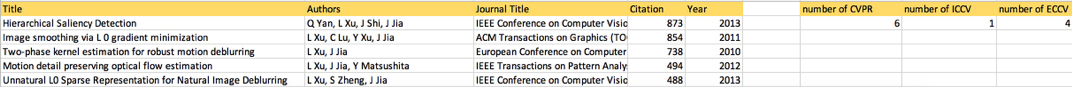
\includegraphics[width=4in]{liu1.png}
  	\caption{Result with EXCEL}
\end{figure}
\begin{figure}[htb]
    \centering
    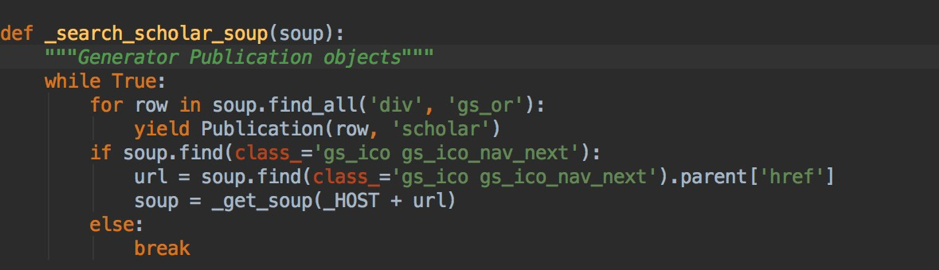
\includegraphics[width=4in]{liu2.png}
  	\caption{Result with Crawler(Part)}
\end{figure}
\begin{figure}[htb]
    \centering
    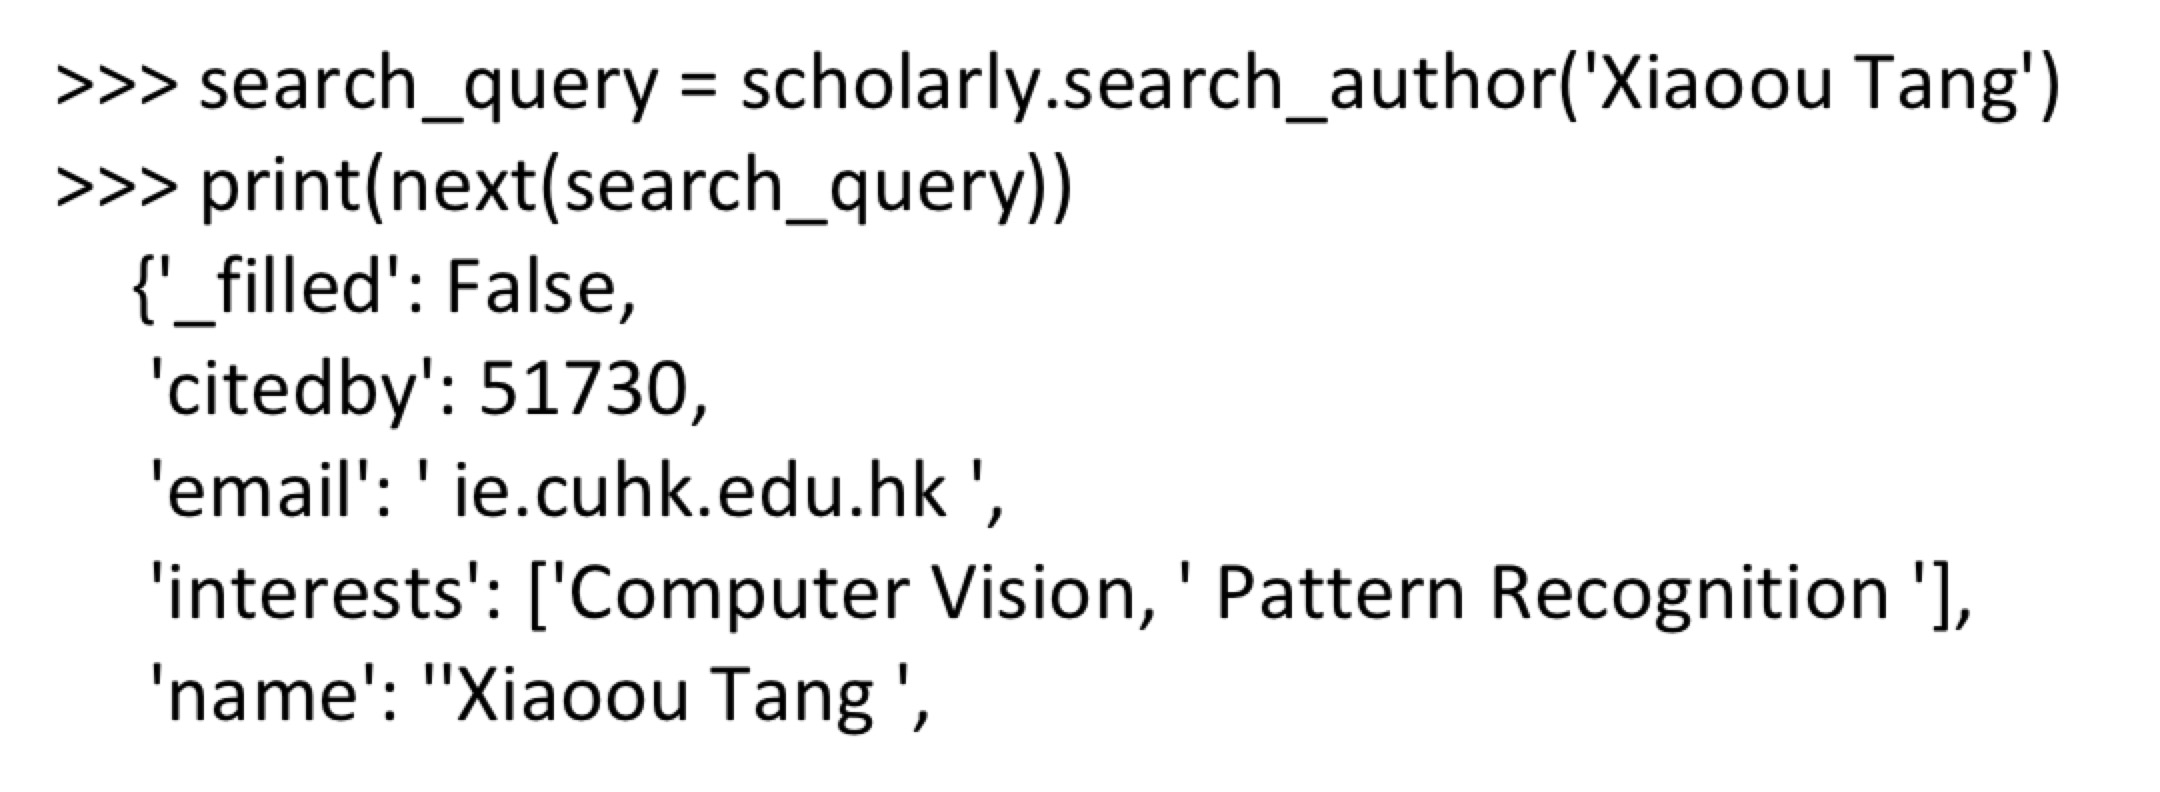
\includegraphics[width=4in]{liu3.png}
  	\caption{Result with Crawler(Part)}
\end{figure}
\subsection{Learning and Progress from the Topic Analyzing Sense Time’s Academic Performance}
In this project, we have chosen Sensetime company as our research target. Our main topic is Using the comments to monitor practicability of products. The core products and services of Sensetime are smart city which include transport hub, real estate, financial security and other 3 aspects, mobile applications, general culture and entertainment, smart healthcare and other aspects in our daily life.  It is hard to cover all the products and services. Therefore, we choose mobile application as our research target. There are two reasons, mobile application is one of representative products of Sensetime and people are more familiar with mobile application. Sensetime focus on the technology of image processing of photo which apply to several mobile phone brands. OPPO is one of famous mobile phone band in China which is a best object of study. 
We have extracted the comments in BaiDu TieBa from Nov. 2017 to Mar. 2019. The main analysis approach is crawling and tabulating the comments, and then dividing the results into two parts: pros and cons. Pros means the positive comments, for example: good, great or others commendatory term, about the camera function, cons means the negative comments such as bad, poor, or other derogatory term. After several times modifications and improvements, we have used NLP in Python to process text information. The idea and method can be divided into 5 steps:
\begin{itemize}
    \item[1.] Word segmentation (using the jieba library to segment Chinese words, because the processing granularity of nltk is generally word, so the text must be segmented first and then treated with nltk. After Chinese word segmentation, the text is a long word composed of each word. Array: [word1, word2, word3... wordn]. You can then use the various methods in nltk to process this text.) 
    \item[2.]Remove the stopwords (create your own nltk Chinese stopword library (download from github)), such as: meaning, derivation, and other meaningless conjunctions.
    \item[3.]Adjust the data format (dict) applicable to the nltk model
    \item[4.]Train the manually classified comments as a training set into the naive Bayesian model.
    \item[5.]Classify data with trained model
    \item[6.]Dividing the result into monthly result 
\end{itemize}
\begin{figure}[htb]
	\centering
	\subfloat[Step 1]{
		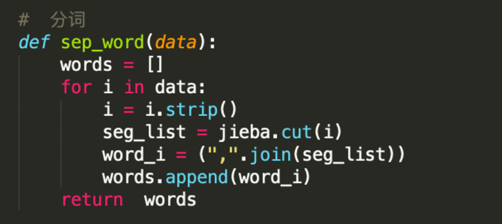
\includegraphics[width=2in]{51.png}}
	%\hspace{0.1in}
	\subfloat[Step 2]{
		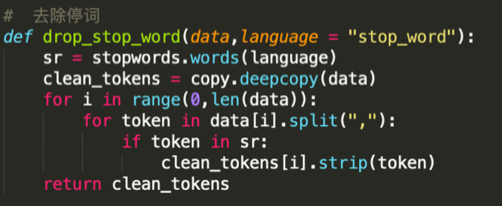
\includegraphics[width=2in]{52.png}}
	%\hspace{0.1in}
	\subfloat[Step 3]{
		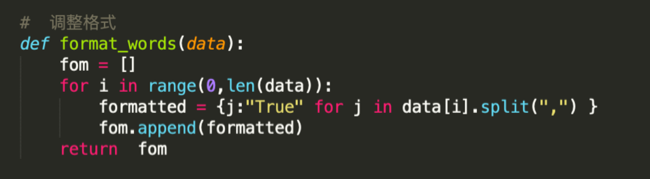
\includegraphics[width=2.5in]{53.png}}
	\caption{The Detail Information of Coding}
\end{figure}
\begin{figure}[htbp]
	\centering
	\subfloat[Step 4]{
		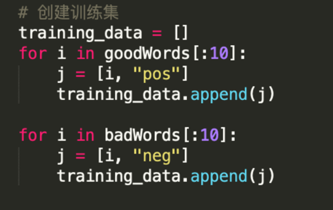
\includegraphics[width=2.5in]{54.png}}
	%\hspace{0.1in}
	\subfloat[Step 5]{
		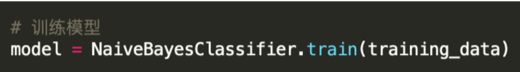
\includegraphics[width=2.5in]{55.png}}
	\caption{The Detail Information of Coding}
\end{figure}
\begin{figure}[!h]
    \centering
    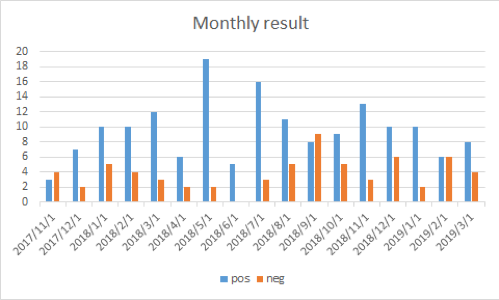
\includegraphics[width=4in]{56.png}
  	\caption{The Final Result}
\end{figure}
\section{Reflection on AI Article}
\subsection{Reflection on the Methodology}
Part two gives a picture of the NLP research. Firstly, the article analysis the bibliographic sources about NLP, which shown an ongoing interest of NLP. Most literature are related to finance, less are related to Accounting, while least are about Audit. Secondly, from chronological perspective, NLP initially started from manual text analysis and then go farther using computer to analysis and mining the data. In late 1990s, we start combine NLP with ML and/or AI. With the internet boomed, the data boomed, too, which make the NLP a necessary. Unique datasets related to target information collecting, analyzing and processing can be done by NLP with ML and/ or AI. When applying NLP into accounting, audit and finance analysis area, plenty of models appears. For example, ANNs, SVMs, DTs, HACM,CLAS, etc. From my point of view, it is the trend that using NLP with ML and/ or AI in analysis accounting, audit and finance. In our case, we can use NLP with ML and/ or AI to monitor the financial statement of the targeting company, also, the big data from digital media such as people’s comments, and reports, news of the targeting company can be collected and analysis by those sophisticated model and algorithm. 
\subsection{Reflection on the Classification}
Nature language process is a useful tool for classifying financial statement content. It has been used to classify and mine these financial documents to obtain insights, make inferences and create other methods and artifacts to improve accounting, auditing and financial knowledge. NLP has been applied to classify the content of Financial Accounting Standards Board (FASB) or the Security and Exchange Commission’s (SEC’s) EDGAR (Electronic Data Gathering, Analysis, and Retrieval) database. NLP is combined with ES (expert system) to create a semantic knowledge base for financial accounting standards (in the Financial Accounting and Reporting System (FARS)). It can improve the accuracy of extract key information in financial statement from 10-K. Besides, a hybrid of rule-based linguistic models and machine-learning techniques (one kind of NLP) and a multi-class support vector machines algorithm can be used to Generate a dictionary financial phrase and general model for assessing the “semantic orientation” (positive, negative or neutral) of financial-related narratives. This can be used to analyze the comments of products from Sense Time. Public comments are essential for product release. According to the concept introduced in the paper, we can base on the past comments of products to build a model for assessing the positive, negative or neutral of comments of the products in the future. It can better monitor and manage the products.  NLP can also be used in information retrieval. Based on the NLP, decision tree and rule-based algorithm to process the journal or article abstract, we can get the required material relatively more accurately. In our project, we have compiled articles from Sense Time executive. However, we met the problems that the number of executive and articles are too many. Our manual search is difficult to achieve comprehensive. This technique could help our project a lot. What’s more, it can classify financial statement content which enable auditors to detect deviations and anomalies in financial statement more effectively. The company can use this technique to improve the quality of financial statement. 
\subsection{Reflection on Prediction}
NLP can be applied in many aspects.It can predict and detect fraud combined with other analysis methods. For example When detecting deceptive emails, the principal is a ‘reduced frequency of first-person pronouns and exclusive words, and elevated frequency of negative emotion words and action verbs’, using singular value decomposition (SVD)-plot analysis.

NLP has been deployed when researchers sought to determine the predictive value of text-based content regarding stock prices, trading volume and exchange rates. Like news-based trading, we can firstly isolate financial news that affects stock prices and/or market activity by a k-NN learning algorithm, then classify textual data associated with upward-trending and downward-trending stock, establishing a predictive relationship between financial news and stock market activity. When we want to use corporate press to predict stock price, we can employ various feature sets such as collection term frequency (CTF), chi-squared (CHI),information gain (IG), and odds ratio (OR)then we can choose various classifiers including linear SVM, Rocchio, k-NN, nonlinear SVM with a Gauss kernel, nonlinear SVM with a sigmoid kernel, and nonlinear SVM with a polynomial kernel. NLP methods have been proved to be effective.in stock prediction.

The fourth part of this natural language processing article combines the specific application of the company's annual report analysis. After reading it, I learned a lot. For example, I learned the effect of combining a lot of algorithms when processing text:
\begin{itemize}
    \item[1.] using TF-IDF term weighting, enhanced with a vector space model classifier, identified significant (p < 0.10) price reactions to MD&A modifications
    \item[2.]Using TF-IDF analysis, augmented with a linear SVM multi-class classification algorithm and the LibSVM regression algorithm (SVR) to identify a significant (p < 0.001) correlation between mandatory annual report disclosures and future firm performance.
    \item[3.]employed keyword counts and thesaurus-based keyword analysis, enhanced with the application of a CART algorithm, to identify text-based variables, improving firm-performance predictions by 5.4%. 
    \item[4.]applied sentiment analysis (using General Inquirer) to small-investor message-board postings.
\end{itemize}
Also, NLP analysis 20 million posts from Live Journal, using two sentiment-classifier algorithms to identify ‘anxious’ posts. ‘The most informative 100 word stems’ were fed to a ‘boosted decision tree’ classifier and identified ‘anxious’ terms ——They demonstrated that social-media postings were significantly (p < 0.01) associated with the equity values of the firms referenced in the postings 
Opinion Finder, which measured positive and negative sentence tone, and Google Profile of Mood States, which measured six mood dimensions, including ‘Calm, Alert, Sure, Vital, Kind, and Happy’. The resulting data set was subjected to Granger Causality analysis and assessment using a self-organizing fuzzy neural network algorithm, predicting changes in the Dow Jones Industrial Average with 87.6 percent accuracy. 
Sentiment expressed in such textual data predicted stock-price changes in Apple, Google, Microsoft and Amazon stock, with accuracy ranging from 75 percent to 82.93percent.
Analysis the data from readability analysis with DT classifiers to categorize messages posted on virtual-investor sites in order to determine the predictive value of postings to such sites. Processing readability data with an SVM algorithm allowed researchers to achieve 62.81 percent accuracy in forecasting stock performance,
Natural language processing is widely used in today's artificial intelligence field. It is becoming more and more important with the deep integration of computer and human life. In the future, I should pay more attention to the simple application of natural language processing.
\section{Synthesis and Suggestions for Future Study}
\subsection{Suggestions for Course}
I choose this course because I am interested in the expertise of artificial intelligence. I advice that you can increase the proportion of expertise of artificial intelligence, set up the examination of professional knowledge etc. Also,this class could give more space for student to show themselves for example, giving speech in the class. 
\subsection{Suggestions for Our Project}
Limited by the lack of  knowledge in computer vision and pattern recognition , we can’t further identify the value  and potential application prospect of the papers. We simply counted the number of papers published on certain journals to evaluate the academic performance of Sense Time. Besides, we have no access to all the staff of Sense Time, the papers we generate can only represent part of Sense Time’s academic performance. So if we have access to more inside information, we can do more analysis such as classifying all the papers into different value-classes or thinking about the potential application to have a more informed view of Sense Time.

\section{Individual Contribution}
\begin{table} [hbp]
    \caption{Individual Contribution} 
    \vspace{10pt}
    \centering
    \begin{tabular}[l]{@{}lcccc}
        \hline
        Group member & Student ID  & AI Article Reflection & Project:Company Research\\  
        \hline
        Jiang Zhining(group leader) &20568072 &Part 3 & Research on product based on comments
        \\
        Zhang YuXin & 20568199 & Part 2	& Research on product based on comments
        \\
        Wan Jing & 20552621	& Part 4.1,4.2,4.3 & Research on company seniors
        \\
        Zhang Lingxi & 20556964 & Part 4.4,4.5,4.6 & Revenue forecast Based on Machine Learning
        \\
        Liu Yifei & 20565678 & Part 5 & Analyzing academic performance
        \\
        \hline
    \end{tabular}  
\end{table} 
\end{document}

